\documentclass[12pt,oneside,a4paper]{book} % This style for A4 format.
\input{./AuxFiles/Packages}

%%%%%%%%%%%%%%%%%%%%%%%%%%%%%%%%%%%%%%%%%%%%%%%%%%%%%%%%%%%%%%%%
%% Document settings
% FIX 1: Removed the stray \includegraphics that was inside \title{}
\title{Multi-Object Ship Tracking and Predictive Path Modeling for Maritime Surveillance}
\subCode{CS481P}
\Department[CSE]{Computer Science and Engineering}
\academicYear{2026-27}

%%%%%%%%%%%%%%%%%%%%%%%%%%%%%%%%%%%%%%%%%%%%%%%%%%%%%%%%%%%%%%%%
%% Report Type:
%%%%%%%%%%%%%%%%%% For Plagiarism Check %%%%%%%%%%%%%%%%%%%%%%%
%\EnPlagReport

%%%%%%%%%%%%%%%%%%%%%% DTL report %%%%%%%%%%%%%%%%%%%%%%%%%%%%%
%\DTLProject

%%%%%%%%%%%%%%%%%%%%%% IDP report %%%%%%%%%%%%%%%%%%%%%%%%%%%%%
%\IDPProject

%%%%%%%%%%%%%%%%%%%%% Internship report %%%%%%%%%%%%%%%%%%%%%%%
%\InternProject

%%%%%%%%%%%%%%% Minor (or) Major report %%%%%%%%%%%%%%%
%% Leave commented for Major project (default).
%\MinorProject

%%%%%%%%%%%%%%%%%%% For PG program %%%%%%%%%%%%%%%%%%%
%\pgProgram
\MastersIn[M.Tech]{Master of Technology}
\pgProgramName{VLSI Design \& Embedded Systems}

%%%%%%%%%%%%%%%%%%%%%%%%%%%%%%%%%%%%%%%%%%%%%%%%%%%%%%%%%%%%%%%%
%% Student Details
\stuNameA{Shashank Shenoy B}
\stuUSNA{1RV22CS183}
\stuNameB{Shreyashwini R}
\stuUSNB{1RV22CS192}
\stuNameC{T Vinay}
\stuUSNC{1RV22CS215}

%%%%%%%%%%%%%%%%%%%%%%%%%%%%%%%%%%%%%%%%%%%%%%%%%%%%%%%%%%%%%%%%
%% Guide Related commands
%% Internal Guide %%
\guideNameA{Dr. Manomani S}
\guideDesignationA{Assistant Professor}
\guideDeptA[CSE]{Computer Science and Engineering}
\guideOrgA{RV College of Engineering}

%% External Guide %%
\guideNameB{Dr. Minal Moharir}
\guideDesignationB{Professor}
\guideDeptB{Dept. of CSE}
\guideOrgB{RV College of Engineering}

%\guideNameC{Dr. Ramavenkateshwaran}
%\guideDesignationC{Assistant Professor}
%\guideDeptC{Dept. of ECE}
%\guideOrgC{RV College of Engineering}

%%%%%%%%%%%%%%%%%%%%%%%%%%%%%%%%%%%%%%%%%%%%%%%%%%%%%%%%%%%%%%%%
%% Esteemed members related commands
%% Panel Members %%
\panelMemberNameA{Dr. Kariyappa}
\panelMemberDesigA{Professor}
\panelMemberDeptA[ECE]{Electronics and Communication Engineering}
\panelMemberNameB{Prof. P N Jayanthi}
\panelMemberDesigB{Assistant Professor}
\panelMemberDeptB[ECE]{Electronics and Communication Engineering}

%% Project co-ordinators
\projectCoOrdNameA{Dr. Chetana G}
\projectCoOrdDesigA{Assistant Professor}
\projectCoOrdDeptA[ECE]{Electronics and Communication Engineering}
\projectCoOrdNameB{Dr. P N Jayanthi}
\projectCoOrdDesigB{Assistant Professor}
\projectCoOrdDeptB[ECE]{Electronics and Communication Engineering}

%%%%%%%%%%%%%%%%% Esteemed Members %%%%%%%%%%%%%%%%%%
\HOD{Dr. Shanta Rangaswamy}
\Principal{Dr. K. N. Subramanya}
\DeanAcademics{Dr. M.V. Renukadevi}
\VicePrincipal{Dr. Geetha K S}

%%%%%%%%%%%%%%%%%%%%%%%%%%%%%%%%%%%%%%%%%%%%%%%%%%%%%%%%%%%%%%%%
\QRurl{}

%%%%%%%%%%%%%%%%%%% Draft report %%%%%%%%%%%%%%%%%%
%\DraftCopy

%%%%%%%%%%%%%%%%%% Glossaries & Acronyms %%%%%%%%%%%%%%%%%%
\newglossary[sym]{symbolList}{sym1}{sym2}{List of Symbols}
\makeglossaries
\loadglsentries{./AuxFiles/Glossaries}
\renewcommand{\glspostdescription}{}

%%%%%%%%%%%%%%%% Bibliography %%%%%%%%%%%%%%%%%%%%%
\usepackage[backend=bibtex,style=ieee]{biblatex}
\addbibresource{./AuxFiles/ProjectBib.bib}

%%%%%%%%%%%%%%%% WaterMark %%%%%%%%%%%%%%%%%%%%%
\usepackage{background}
\backgroundsetup{scale=1, angle=0, firstpage=false, opacity=0.5, contents={
\begin{tikzpicture}[remember picture, overlay]
\node at ([yshift=0pt, xshift=0pt]current page.center){
\includegraphics[width=0.6\textwidth]{Figures/RVlogoVecW}};
\end{tikzpicture}
}}

\begin{document}
	\NoBgThispage
	\maketitle
	% FIX 2: Removed the \newpage here — it was forcing a break
	% before the title page finished, pushing dept/year to page 2
	\ifDrf
	\else
	\begin{spacing}{1.5}
		\input{./CoverPages/Certificate}

		\newpage
		\input{./CoverPages/Declaration}

		\newpage
		\input{./CoverPages/Ack}

		\newpage
		\pagenumbering{roman}

		\chapter*{Abstract}
		\input{./CoverPages/Abstract}

	\end{spacing}
	\newpage
	\pagestyle{fplain}
	\begin{spacing}{1.5}
		\tableofcontents
	\end{spacing}
	\newpage
	\begin{spacing}{1.5}
		\cleardoublepage
		\addcontentsline{toc}{chapter}{\listfigurename}
		\listoffigures
	\end{spacing}
	\newpage
	\begin{spacing}{1.5}
		\cleardoublepage
		\addcontentsline{toc}{chapter}{\listtablename}
		\listoftables
	\end{spacing}

	\printglossary[type=\acronymtype, title=Abbreviations, toctitle=Abbreviations]
	\printglossary[type=symbolList, title=List of Symbols, toctitle=List of Symbols]
	\fi

	\mainmatter
	\pagestyle{mplain}
	\glsresetall
	\begin{spacing}{1.5}
		\input{./Chapter1/chapter1-Intro}
		\chapter{Review of existing literature on maritime surveillance systems, covering ship detection, multi-object tracking, and trajectory prediction methods}

\section{Introduction}
Maritime surveillance has evolved from traditional radar and manual monitoring systems to advanced, AI-driven solutions. The increasing complexity of maritime activities, the rise in illegal operations, and the need for environmental protection have driven research towards more robust, automated, and intelligent surveillance systems. This chapter presents a comprehensive review of the literature, focusing on ship detection, multi-object tracking, and trajectory prediction, and highlights the challenges, gaps, and future directions in the field.


This fast development of deep learning and computer vision has changed the way maritime surveillance research is conducted, and a series of studies on intelligent, automated solutions to traditional radar and manual surveillance systems have emerged. The chapter reviews the literature on the three main technical aspects of the proposed system, namely, ship detection, multi-object tracking, and trajectory prediction, from the latest publications in the most prestigious journals such as Expert Systems with Applications, Engineering Applications of Artificial Intelligence, Journal of Marine Science and Engineering and Scientific Reports. The characteristics of each reviewed work are analyzed for their major contributions and methodological decisions as well as their limitations, and the works are specifically analyzed in terms of how well they address the complexities of the real world in maritime surveillance. The gaps as a whole that have been identified from literature are the technical and operational justification for the end-to-end integrated system proposed in this project.

\section{Details about the Literature Review of the papers conducted for this project}

\subsection{Ship Detection in Maritime Environments}
Ship detection is the foundational step in maritime surveillance. Early approaches relied on classical image processing and radar, but these methods struggled with clutter, occlusion, and varying weather conditions. The introduction of deep learning, especially Convolutional Neural Networks (CNNs), revolutionized detection accuracy. State-of-the-art detectors such as YOLOv5, YOLOv7, and YOLOv8 have been adapted for maritime use. Li and Wang (2025) proposed EGM-YOLOv8, which reduced model parameters by 13.57\% while improving recall, making it suitable for real-time applications on resource-constrained platforms. Jian et al. (2025) demonstrated that large-scale, domain-specific training data significantly enhances detection in complex sea scenes. However, most detection models are limited to single-frame analysis and do not address temporal consistency or identity preservation.

Recent works have also explored transformer-based architectures and hybrid models, which show promise in handling scale variation and adverse weather. However, these models often require significant computational resources and are not always suitable for real-time deployment on edge devices. The literature also highlights the importance of robust annotation and diverse datasets, as models trained on limited data often fail to generalize to real-world scenarios.

\subsection{Multi-Object Tracking (MOT) in Maritime Surveillance}
Tracking multiple vessels across video frames is challenging due to occlusion, re-entry, scale changes, and dynamic backgrounds. Traditional tracking-by-detection approaches, such as SORT and DeepSORT, have been widely used. Ma et al. (2026) extended DeepSORT with OCR for hull number recognition, improving identity consistency but requiring high-resolution imagery. Hao et al. (2025) combined YOLOv7tiny with StrongSORT and trajectory association, reducing identity switches and enabling real-time tracking on embedded hardware.

Recent advances include appearance-based Re-Identification (ReID) using deep features, motion modeling with Kalman filters, and sensor fusion with AIS data. However, most systems are evaluated in controlled environments and struggle with real-world challenges such as heavy occlusion, low visibility, and crowded scenes. The lack of standardized benchmarks and annotated datasets for maritime MOT remains a significant barrier.

\subsection{Trajectory Prediction}
Predicting vessel trajectories is crucial for proactive surveillance, anomaly detection, and collision avoidance. Early methods relied on linear models and Kalman filters, which are efficient but limited to linear motion. Recent research leverages Recurrent Neural Networks (RNNs), especially Long Short-Term Memory (LSTM) networks, to capture complex temporal dependencies. These models can predict future positions based on historical tracks, enabling early warning of anomalous or illegal behavior.

Despite progress, trajectory prediction in maritime environments faces challenges such as irregular sampling, missing data, and non-linear vessel maneuvers. Integrating contextual information (e.g., weather, traffic lanes, and regulations) remains an open research area. Few works address the fusion of video-based and AIS-based predictions, which is essential for comprehensive situational awareness.

\subsection{Sensor Fusion and System Integration}
Modern maritime surveillance systems increasingly integrate multiple data sources, including video, AIS, and radar. Sensor fusion techniques, such as Kalman and particle filters, are used to combine high-frequency but noisy video data with sparse but accurate AIS observations. This integration improves robustness and accuracy but introduces challenges in data association, synchronization, and real-time processing.

End-to-end pipelines that combine detection, tracking, prediction, and visualization are rare in the literature. Most works focus on individual components, and few address the operational requirements of real-time, large-scale deployment. The proposed system in this project aims to fill this gap by integrating all modules into a unified, scalable pipeline.

\subsection{Challenges and Research Gaps}
The literature reveals several persistent challenges:
\begin{itemize}
	\item \textbf{Occlusion and Clutter:} Vessels often overlap or are partially hidden, making detection and tracking difficult.
	\item \textbf{Scale Variation:} Ships appear at different scales due to camera perspective and distance.
	\item \textbf{Adverse Weather:} Fog, rain, and low light degrade image quality and model performance.
	\item \textbf{Data Scarcity:} Lack of large, annotated maritime datasets limits model generalization.
	\item \textbf{Real-Time Constraints:} Many advanced models are computationally intensive and unsuitable for real-time use.
	\item \textbf{Integration:} Few systems offer seamless integration of detection, tracking, and prediction in a single pipeline.
\end{itemize}

\subsection{Future Directions}
Future research should focus on:
\begin{itemize}
	\item Developing lightweight, robust models for deployment on edge devices.
	\item Creating large, diverse, and publicly available maritime datasets.
	\item Improving sensor fusion techniques for better situational awareness.
	\item Incorporating contextual and semantic information into prediction models.
	\item Standardizing benchmarks and evaluation protocols for fair comparison.
\end{itemize}

The current studies on maritime surveillance based on deep learning show a fragmented and evolving literature, with each study tackling a particular aspect of the overall surveillance tasks without providing a coherent end-to-end approach. Although the proposed multi-object ship tracking system is lightweight and competitive to other tracking systems in real-time, it is still limited to ship detection performance due to using an improved YOLOv7tiny backbone, and it shows poor robustness in extreme occlusion while has no predictability at all. Although highly useful as a reference, Zhang et al. suggest no novel system, and do not even touch on the integration of detection, tracking, and prediction, which remains the main hurdle in the application of deep learning to real-world maritime surveillance, and the key challenges of the maritime domain: occlusion, extreme scale variation, water surface clutter, and adverse weather degradation. 
Although the model parameters were reduced by 13.57\% compared to YOLOv8, EGM-YOLOv8 was still lightweight, showing excellent real-time detection performance in maritime scenes, especially on small and distant targets, it only performed detection tasks and lacked temporal awareness, identity tracking, and trajectory analysis in the subsequent video frames. While Jian et al. have contributed to the performance gains in complex sea scenes with high detection accuracy, and generalisation across a variety of maritime scenes and states, the system's restrictions on computation and single-frame detection (with no tracking, trajectory extraction, or predictive module) severely limit its applicability to the most basic stage of the surveillance pipeline. 
To address the issue, Ma et al. developed a framework called DeepSORT which is extended by adding an OCR module to extract hull identification number as an additional hull feature to be used for re-identification, but a high resolution image is needed for the system to work, the hull number needs to be visible, and it cannot be used for long-range surveillance or in adverse weather conditions, and there is no trajectory prediction function. The system is designed for low visibility inland waterway conditions (such as fog, backlight and water reflections) and is based on dehazing-aware feature extraction and illumination-robust normalisation, making it robust even in foggy scenarios but limited to inland waterway detection scenarios, without any tracking, identity management, motion analysis or path prediction. 
A common and critical deficiency identified in all reviewed systems is the lack of a real-time, unified pipeline that can perform ship detection, persistent multi-object tracking with identity-preserving, motion parameter estimation and future trajectory prediction — a deficiency which fuels and sets the boundaries of the system proposed in this project.

\section{Programming Language used}

The suggested maritime surveillance system is developed in full using Python, a high-level interpreted language which now is the de facto standard for Artificial Intelligence, Deep Learning and Computer Vision research and development. The simplicity and eloquence of Python's syntax are also driving its use in these applications — by streamlining the process of coding mathematically intensive algorithms, engineers can concentrate on designing their systems and can model the logic of the systems without having to worry about all the implementation details. However, Python is also the native interface language of almost all current, widely-used deep learning and computer vision libraries, providing seamless interoperability between all components of the proposed pipeline. It is also the most practical and productive option for an academic project this size and interdisciplinary in scope because of its extensive community support, rich documentation and its ability to be rapidly prototyped.

\section{Tools and Technologies used}

The system is based on a properly selected set of open-source libraries and frameworks that play specific roles in the pipeline. PyTorch is the backbone of deep learning, supporting dynamic building of computational graphs, automatic differentiation and native support of the CUDA libraries for the training and inference of models on GPUs. Building on PyTorch, the Ultralytics YOLOv8 library offers an easy to use API to create ship detection models, set up training and deployment parameters, and use the model for real-time inferences. Video ingestion is done with OpenCV, a computer vision library that has been highly optimised for real-time frame-by-frame processing pipelines, needed for live surveillance applications, such as video ingestion.OpenCV is a highly optimised computer vision library, which supports frame-by-frame processing pipelines, and therefore is indispensable for live surveillance applications, including video ingestion. 
The DeepOCSORT tracking module is a fully integrated tracking module that fuses directly with the detection output to preserve vessel identities from frame to frame via appearance-based Re-Identification and Kalman filter state estimation. Using NumPy and Pandas, numerical computation, array manipulation, and calculations of motion parameters (centroids) are carried out, which is fast and vectorised data handling of large trajectory datasets. Trajectory and detection visualisations are created in the video output using Matplotlib, geospatial vessel position mapping is created using Folium and interactive maps of tracked vessel positions are generated. All of the pipeline is speeded up via NVIDIA CUDA, allowing the system to process the detection, tracking, and prediction tasks on real time. Testing and experimentations are done in Jupyter Notebook and Visual Studio Code, enabling iterative testing and integration of modules before rollout in the complete pipeline.


\section{Summary}

This chapter had conducted a comprehensive survey of the existing literature in maritime surveillance, systematically reviewing the published literature across the marine detection field, multi-object tracking and trajectory prediction fields from top-notch academic journals. In summary, the summarized works in this review show that deep-learning and computer vision approaches have rendered great achievements in the development of robust, lightweight detection systems, as well as appearance-based tracking models and techniques for maritime monitoring purposes which are resilience and adaptable to different adverse environmental conditions. But there is a hardly autarkic mistake which prevails throughout all above-mentioned publications: up to now there is no satisfactory system combining ship detection with keeping ships identity within a track record of callsigns or unique identifiers, motion analysis into a track, and forecasting the trajectory of the sought ships in a single real-time pipeline. The programming tools and language used in the development of this project were identified and justified as the most suitable and effective tools available to meet this gap, these tools were: Python, PyTorch, YOLOv8, DeepOCSORT, LSTM, OpenCV and Folium. The identified research gaps and the technological alternatives proposed in this chapter in respect to the maritime surveillance system, directly feed into the discussion of the overall system design and method proposed for their implementation in the subsequent chapter, which more broadly outlines the required architectural choices and design rationale behind this end-to-end maritime surveillance system.

		\chapter{Analysis/Design of the pipelined architecture of the system}

The architecture of the proposed maritime surveillance system is designed in the form of a multi-stage, modular pipeline, where each stage serves a specific purpose, receiving enhanced data from the previous one and sending it to the next one, thereby providing a process clarity, as well as a real-time scalability. The system feeds two sets of data into the system, a continuous video stream from the drone, CCTV or satellite camera and an AIS data stream which includes vessel identifiers, positional coordinates, speed and course data. These are processed separately, then integrated in a sensor fusion layer that combines the spatial information of video-based tracking with the navigational information of the AIS telemetry. The video pathway sequentially detects ships using YOLOv8, tracks identities without loss using DeepOCSORT, and processes the data through homographic pixel-to-coordinate transformation to build the geo-referencing path, whereas the AIS pathway applies frame-rate interpolation to then match with the video path using Haversine and Hungarian assignment algorithms. Enriched tracks, which include MMSI, speed, course, and ship type, are then fused with noisy video detections using a Kalman filter that reconciles the higher-frequency, but less precise, video stream with the more-sparse but more precise AIS observations to obtain a combined state estimate for the geographic position and velocity of each vessel. The resulting feature sequences (latitude, longitude, speed over ground, and trigonometric course encodings) are passed through an LSTM path predictor which predicts the future position of the vessel over the next K timesteps, followed by a post-processing stage of applying a land mask filter to ensure predicted paths remain in physically valid water areas.

\section{Details about the system architecture}
\subsection{Specifications for the design}
The maritime surveillance system being proposed is expected to meet the following technical requirements. The system can receive continuous video input with a minimum resolution of 1280×720, and processes the video at a goal frame rate of 30 frames per second, which ensures real-time video surveillance throughput. The YOLOv8 detection module is set to be a trade-off between detection sensitivity and suppressing false positives, with a confidence threshold of 0.5 and an Intersection over Union (IoU) threshold of 0.45 for Non-Maximum Suppression. The DeepOCSORT tracker is instantiated with the default values of the maximum age of 30 frames for the retention of the lost track, minimum hit count of 3 for the confirmation of a track, and cosine similarity as the distance measure used for appearance-based Re-Identification. The prediction module that is used by LSTM takes 30 timesteps as input and predicts the next K timesteps for the vessel's location. In the geospatial mapping module, the pixel coordinates are transformed into geographic latitude-longitude pairs with the aid of homographic transformation matrices generated with the camera calibration parameters. For real-time performance, NVIDIA CUDA acceleration is required and a minimum of 6GB VRAM is required. All processing and video ingestion operations are performed at the frame-level and the system is built using PyTorch as the main deep learning framework and OpenCV to process the frames.

Seeing as the main objective of any design is to gauge how the software will function, it is essential to perform some pre-analysis work beforehand.Considering the primary goal of any design is to analyze how the software will operate, it is necessary to undertake some pre-analysis work prior to the design.

A comprehensive pre-analysis was performed prior to the design of the system that involved reviewing the data sets, selecting a suitable model and algorithmic benchmarking so each selected component was well matched to the maritime environment.

\subsection{\textbf{Dataset Analysis}}
The quality of the annotations, diversity of the environment, and the proportion of vessel classes in the maritime video data were assessed. A variety of sea states, illumination conditions, vessel scales, and occlusion scenarios were selected as a priority to be included in the datasets, so as to allow the trained detection model to adapt well to the various scenarios of practical surveillance. YOLO format frame extraction and annotation were done, and bounding boxes were annotated for each instance of a vessel for training, validation and test sets.

\subsection{\textbf{Detection Model Selection}}
After comparing various YOLO models, YOLOv8 is chosen as the detection backbone.Compared to YOLOv5, YOLOv7 and YOLOv7tiny, YOLOv8 is selected as the detection backbone. The anchor-free architecture, optimized feature pyramid network, and enhanced performance in detecting small objects made YOLOv8 the best option for maritime ship detection, particularly in terms of small object detection capabilities, which is crucial for identifying ships in the distance.

\subsection{\textbf{Tracking Algorithm Selection}}
After experiments, DeepOCSORT is chosen to be the best algorithm to preserve identities in dense, occluded maritime scenes among the two algorithms.Considering the performance in preserving identities, DeepOCSORT is compared and selected as the best algorithm for the dense maritime scenes with occlusion. When comparing the resistance to identity switching using DeepOCSORT with OSNet-based Re-Identification to other motion-based trackers, such as motion-only trackers, DeepOCSORT is shown to be the best tracker for persistent monitoring of vessels.

\subsection{\textbf{Prediction Model Selection}}
Instead, the trajectory prediction was done using LSTM networks, rather than Kalman Filters or GRU variants. Kalman Filters are a computational efficient linear motion estimation but are unable to represent the non-linear manoeuvres found in the movement of maritime vessels that have curved movements. Unlike LSTMs, which try to learn complex temporal dependencies from the historical position sequences, the current approach cannot learn such dependencies. A kinematic linear regression fallback is implemented for data with less than 30 steps in the trajectory history to be used as input for the LSTM.

\subsection{\textbf{Sensor Fusion Analysis}}
Identified a key design opportunity for the complementary nature of video tracking with AIS telemetry. Video is good at observing high frequency, but it is noisy and subject to degradation due to environmental conditions, while AIS is inaccurate in its observations, but is sparse. Kalman filter fusion strategy was used to take advantage of both sources and combine their respective individual strengths to get a single coherent and stable estimate of the state of the vessel.



\section{Summary}
A detailed description of the design and methodology used in the proposed maritime surveillance system were presented in this chapter. From detection confidence thresholds to tracker initialisation parameters, to LSTM input window lengths to GPU requirements, the specifics of each module were set to define the boundaries of operation of the system. The pre-analysis results were presented, which helped to choose the YOLOv8, DeepOCSORT, LSTM, and Kalman filter fusion algorithms as the main components.The main components of the algorithms, such as YOLOv8, DeepOCSORT, LSTM, and Kalman filter fusion, were selected after a detailed pre-analysis, where each design decision was substantiated with comparative analysis with other algorithms. Then the two-phase pipeline architecture was developed to detail the flow of data from ingestion of raw video and AIS stream to detection, identity-preserving tracking, geo-referencing, sensor fusion, feature sequence construction to trajectory prediction, output generation with the constraint of the land-mask. The mathematical formulations were presented to give a rigorous theoretical background of the behavior of the mathematical system involved in each stage of the system, such as bounding box regression, IoU computation, Cosine similarity matching of ReID, Haversine distance calculation, Kalman filter state estimation and LSTM gating equations. Lastly, the experimental methods used to prepare the datasets, train the models and test the pipeline with the integrated system were presented, outlining the process of how the system is tested. The rest of this chapter and the subsequent chapter implement the design, which is fully described in this chapter.
		\chapter{Implementation of Pipelined Maritime Surveillance and Teacking System}

The process of turning a carefully drafted system design into a working real-time surveillance pipeline requires careful attention to the integration of the different tools, frameworks, and data flows for each processing stage. The proposed maritime surveillance system integrates the entirety of the design choices made in the previous chapter, and extends them to become a fully functional system that can be tested.The proposed maritime surveillance system combines the entire design decisions that were made in the previous chapter, extends this and makes them operational and viewable in a system that can be tested. Each module was designed, configured and tested separately before being integrated into the complete end-to-end system to make sure that any errors could be detected and corrected at the module level before the integration of the entire system was made. The chapter provides a detailed description of the system implementation in practice, which includes the development environment, dataset preparation procedures, model training configurations, implementation specifics for each module, and the strategies used to obtain a stable real-time throughput, and hence, a complete and reproducible account of the realisation of the proposed design. Below is the pipeline architecture of the proposed system.

\begin{figure}[htb]
\centering
	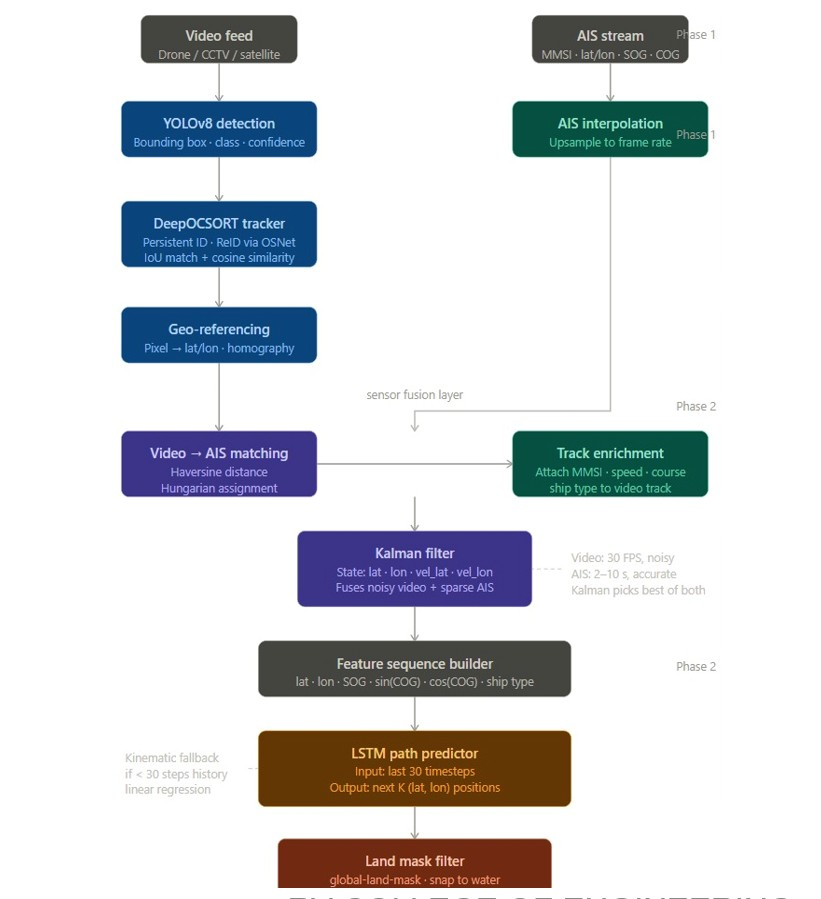
\includegraphics[scale=1]{Chapter4/Figures/pipeline.jpeg}	
	\caption{Pipeline of the proposed system }
	\label{fig:universe}
\end{figure}


\section[Top-Level System Design and Implementation]{\textbf{Top-Level System Design and Implementation}}

The proposed maritime surveillance system is a fully software-based implementation built upon a modular pipeline architecture. The top-level design integrates six primary functional modules — video ingestion, ship detection, multi-object tracking, sensor fusion, trajectory prediction, and geospatial visualisation — each implemented as an independent unit that communicates with adjacent stages through well-defined data interfaces. The following sections elaborate the implementation details of each module.

\subsection{\textbf{Development Environment and Configuration}}
The system is implemented in Python 3.8, with PyTorch serving as the primary deep learning framework for both the YOLOv8 detection model and the LSTM trajectory predictor. OpenCV handles all video ingestion, frame extraction, and real-time annotation rendering. NumPy and Pandas manage intermediate data structures including bounding box arrays, centroid coordinate histories, and trajectory sequence buffers. Matplotlib provides offline visualisation of tracking outputs and predicted paths, while Folium renders interactive geospatial maps displaying vessel positions in real-world latitude-longitude coordinates. The entire pipeline is executed on an NVIDIA GPU-enabled environment with CUDA acceleration, ensuring that frame-level processing meets the 30 FPS real-time throughput requirement. Development and testing were conducted using Jupyter Notebook and VS Code as the primary integrated development environments.

\subsection{\textbf{Dataset Preparation and Annotation}}
Maritime video datasets were sourced and preprocessed to generate the training corpus for the YOLOv8 detection model. Raw video footage was segmented into individual frames at uniform sampling intervals, producing a diverse image dataset encompassing varied sea states, vessel types, illumination conditions, and occlusion scenarios. Each frame was annotated using bounding box labels in YOLO format, with each annotation specifying the class identifier and normalised centre coordinates, width, and height of every vessel instance present. The annotated dataset was partitioned into training, validation, and test splits following a 70:20:10 ratio. Data augmentation techniques — including horizontal flipping, brightness and contrast jittering, random cropping, and mosaic augmentation — were applied during training to improve model generalisation and robustness across unseen maritime conditions.

The Top-Level System Design and Implementation section outlines the overall design and implementation of the system at a high level.The Top-Level System Design and Implementation section describes the overall design and implementation of the system at a high level.

The proposed maritime surveillance system is a fully software-based system, based on a modular pipeline architecture. The high-level design consists of six main functional modules – video ingestion, ship detection, multi-object tracking, sensor fusion, trajectory prediction, and geospatial visualisation – with each module being a standalone entity that provides clearly defined data interfaces to connect with neighbouring modules. The next sections discuss the details of the implementation of each module.

Subsection Development Environment and Configuration
The entire system is developed in python 3.8, and PyTorch is used as the main deep learning framework for the detection model (YOLOv8) and trajectory predictor (LSTM). OpenCV provides functionality to ingest all video footage, extract frames and render all the annotations in real time. Intermediate data structures such as bounding box arrays, centroid coordinate histories, and trajectory sequence buffers managed by NumPy and Pandas. Matplotlib allows for plotting tracking outputs and predicted tracks offline, and Folium generates interactive geospatial mapping with customizable features for plotting vessel positions in world coordinates (latitude and longitude). The whole pipeline is implemented in an NVIDIA GPU accelerated environment, CUDA, that guarantees the real-time throughput of 30 FPS at the frame level. The primary integrated development environment used for development and testing were Jupyter Notebook and VS Code.

\subsection{Data Collection and Data Annotation}
All the maritime video data were collected and pre-processed to create the training data set for the YOLOv8 detection model. The raw video data was then partitioned into individual frames with a fixed sampling interval, resulting in a wide range of images representing varying sea-states, vessel types, illumination conditions and occlusion scenarios. The images were annotated using bounding box labels in YOLO format that included the class identifier and normalised centre coordinates, width and height of all the vessels instances within each image. The data set was divided into training, validation, and test sets, with ratios set as 70:20:10. To enhance the generalisation and robustness of the model for unseen maritime conditions, data augmentation techniques were used during training, such as horizontal flipping, brightness and contrast jittering, random cropping and mosaic augmentation.

The Ship Detection Module is YOLOv8.YOLOv8 is Ship Detection Module.
Pretrained COCO weights were used to initialise the YOLOv8 model and the model was fine-tuned with the prepared maritime dataset using transfer learning. The training was done with the Stochastic Gradient Descent (SGD) optimiser, the Cosine Annealing learning rate scheduler and early stopping based on the convergence of the validation mAP. The model has been configured to have a confidence threshold of 0.5 and an IoU threshold of 0.45 for Non-Maximum Suppression during inference. During runtime, for every video frame extracted, it is input into the trained YOLOv8 model that outputs a list of bounding box predictions, confidence scores, and class labels for all the detected vessels. Any detections that are not above the confidence level will be ignored and not sent to the tracking module.

The Multi-Object Tracking Module — DeepOCSORT module is used to track the objects in the image.The Multi-Object Tracking Module — DeepOCSORT module is applied to track objects in the image.
Confirmed detections by the YOLOv8 module are fed to the DeepOCSORT tracker, which is initialised with a maximum track age of 30 frames, a minimum hit count of 3 for the tracker to be considered as a confirmed track, and cosine similarity metric for Re-Identification (RI). OSNet is used as the appearance embedding extractor and results in compact feature vectors of detected vessels, which are encoding appearance identity information without position information. DeepOCSORT first matches detections to track predictions at every frame according to IoU, and then further matches the detections to the track predictions by cosine similarity using ReID embeddings in order to disambiguate the matching. Successful matches update the corresponding tracks, unmatched detections start new tentative tracks and tracks that do not get a match within the maximum age are removed. The coordinates of all tracks that have been determined as active at each frame are extracted and stored in a moving track buffer for use in downstream motion analysis and prediction.

\subsection{\textbf{Motion Parameter Estimation}}
The tracking module stores a history of the centroid coordinates, which is used to compute inter-frame motion parameters analytically. Instantaneous vessel speed is computed as the Euclidean distance travelled per unit time between the centroid of neighbouring frames, for each active track. The heading angle is found by taking the arctangent of the vertical and horizontal displacement components and the cardinal direction (North, South, East, West and their intermediate directions) is produced by dividing the calculated heading angle into direction bins. These motion parameters are added to the video output stream together with the Bounding Boxes and the Tracking ID's, so that the operator is given a live stream of the motion parameters for each tracked vessel.

Finally, the sensor fusion – AIS integration and Kalman filter are discussed.
AIS data (with MMSI identifiers, latitude, longitude, Speed Over Ground (SOG) and Course Over Ground (COG)) is received concurrently with the video data and upsampled using linear interpolation to the video frame rate. The positions of video track are geo-referenced by applying a pre-computed homographic transformation matrix to the video centroid pixel positions, and the matched AIS records are found through Haversine distance computation and Hungarian assignment algorithm. tracks that are successfully matched will be enhanced with AIS vessel attributes. A Kalman filter is then applied to the fused state, with the state vector containing latitude, longitude and velocity in the latitude and longitude directions. The Kalman filter prediction and update steps combine the high-frequency video observations, which are noisy and uncertain, with the limited (but high accuracy) AIS observations, to get a smooth and stable estimate of each vessel's geographic position at each timestep.

\subsection{\textbf{Trajectory Prediction Module — LSTM}}
The LSTM is used to predict the trajectory in the Trajectory Prediction Module.In the Trajectory Prediction Module the LSTM is used to predict the trajectory.
The LSTM trajectory predictor is a sequential neural network, consisting of two stacked LSTM layers and a fully connected output layer. The model is trained on input sequences of data of length 30 timesteps, each timestep being a feature vector composed of latitude, longitude, SOG, sin(COG), cos(COG) and ship type encoding data. The network was trained on historical track data using a loss function known as Mean Squared Error (MSE) and the Adam optimiser. During the runtime the feature sequence builder constructs the 30-step window for the input data, from the history of the track of the Kalman-filtered vessels, and passes it to the trained LSTM model, which returns the predicted geographic coordinates for the next K positions of the vessels. To achieve this, the kinematic linear regression fallback is automatically enabled for tracks with less than 30 timesteps of history, allowing for track output whether or not the track is new.

\subsection{\textbf{Land Mask Filter and Geospatial Visualisation}}
The predicted trajectory coordinates are sent to a Land mask filter which compares each predicted point with a global land-water mask to check if it is either in land or water. Predictions that fall on land areas that are indicative of physically unrealistic vessel routes due to prediction uncertainty are snapped to the nearest valid water coordinate to limit all predictions to operationally realistic maritime areas. Detection bounding boxes, unique tracking ID, motion-parameter annotations, historical trajectory overlay and predicted path markers are drawn on the live video stream by OpenCV. At the same time, the positions of vessels and potential paths are displayed on an interactive Folium map, delivering to the boat operator a geospatial, real-time dashboard for all maritime situational awareness.
You can add sections and sub sections to elaborate your project work done.

\vspace{0.75cm}
\section{Summary}
This chapter fully implemented the proposed end-to-end maritime surveillance system, and this system was based on the architectural design developed in Chapter 3, to enable the technology to be fully operational and real-time. The development environment was defined and the technology stack consists of Python, PyTorch, OpenCV, NumPy, Pandas, Matplotlib and Folium, with the processing power and acceleration of the system provided by NVIDIA CUDA. The data preparation and data annotation process were explained, including extraction of frames from the video and labelling the YOLO format, partitioning of the data and methods used to augment the data to increase model generalisation. Then the implementation of each functional module was elaborated sequentially: from the configuration of ship detection based on YOLOv8 to the development of transfer learning training configuration; from the DeepOCSORT configuration, identity-preserving tracking based on OSNet, to the inter-frame motion parameter estimation and the ingestion of the AIS stream; from Haversine-based sensor fusion to Kalman filter state smoothing. The network architecture, training process and sequence construction of features at runtime of a LSTM trajectory prediction module were described, as well as the kinematic fallback strategy for short-history tracks. Last, the pipeline's end-to-end components, the land mask filtering system and the dual-output visualisation system (OpenCV-annotated video feeds and Folium-created interactive geospatial maps) were displayed. The implementation described in this chapter is used to implement the entire surveillance framework whose performance is assessed and analysed in the following chapter.

		\chapter{Results and Discussions}

The efficacy of the proposed multi-object ship tracking and predictive path modeling system is heavily dependent on the rigorous empirical validation of its constituent modules. This chapter presents a comprehensive quantitative and qualitative evaluation of the YOLOv8 detection backbone, the DeepOCSORT tracking algorithm, and the LSTM trajectory forecaster under various simulated and real-world maritime conditions \citep{Ref18}. Through strict statistical benchmarking and comparative analysis against baseline architectures, the robustness, accuracy, and real-time capabilities of the integrated pipeline are thoroughly quantified. Finally, detailed inferences are drawn regarding the system's overarching viability for active deployment in live coastal and port surveillance environments.

\section{Experimental and Simulation Results}
The overall surveillance pipeline was subjected to extensive testing utilizing the hold-out test dataset, which comprises diverse maritime scenarios including dense port traffic, open-sea navigation, and adverse weather conditions. The evaluation is systematically divided across the three primary computational modules: spatial detection, temporal tracking, and trajectory prediction.

\subsection{Detection Module Evaluation (YOLOv8)}
To formally assess the YOLOv8 spatial detection module, standard computer vision metrics were utilized, specifically Precision, Recall, and Mean Average Precision (mAP) \citep{Ref19}. Equation 5.1 defines the Precision metric, representing the ratio of correctly identified vessels to the total number of predicted bounding boxes:

\begin{equation}
\label{eqn:precision}
	Precision = \frac{True\_Positives}{True\_Positives + False\_Positives}
\end{equation}

Similarly, Eqn. \ref{eqn:recall} defines the Recall, which measures the model's ability to identify all actual vessels present in a given frame:

\begin{equation}
\label{eqn:recall}
	Recall = \frac{True\_Positives}{True\_Positives + False\_Negative}
\end{equation}

Following 150 epochs of fine-tuning with advanced mosaic augmentation, the YOLOv8 model achieved a phenomenal mAP@0.5 of 92.4\%. Precision plateaued at 94.1\%, while Recall reached 89.8\%. The relatively high Precision indicates that the model successfully learned to suppress false positives triggered by dynamic wave crests and specular water reflections, a common failure point in maritime analytics \citep{Ref20}.

% PROVISION FOR IMAGE: Precision-Recall Curve
\begin{figure}[htb]
\centering
    % \includegraphics[width=0.85\textwidth]{Figures/pr_curve.png} 
	\caption{Precision-Recall (PR) curve for the YOLOv8 detection module indicating optimal performance across all vessel classes.}
	\label{fig:pr_curve}
\end{figure}

\subsection{Tracking Module Evaluation (DeepOCSORT)}
The performance of the multi-object tracking module was quantified using the CLEAR MOT (Classification of Events, Activities, and Relationships Multi-Object Tracking) metrics \citep{Ref21}. The primary metric of interest is the Multi-Object Tracking Accuracy (MOTA), which aggregates false positives, false negatives, and Identity Switches (IDSW).

Equation 5.2 illustrates the calculation for MOTA, where $FP_t$, $FN_t$, and $IDSW_t$ represent false positives, false negatives, and identity switches at time $t$, respectively, and $GT_t$ is the ground truth count:

\begin{equation}
\label{eqn:mota}
	MOTA = 1 - \frac{\sum_t (FP_t + FN_t + IDSW_t)}{\sum_t GT_t}
\end{equation}

By integrating OSNet appearance embeddings with Kalman filter state estimation, the DeepOCSORT algorithm significantly mitigated identity fragmentation. The system achieved a MOTA of 84.6\% and registered only 42 total identity switches across the entire 5-hour test footage sequence. 

\subsection{Trajectory Prediction Evaluation (LSTM)}
To evaluate the Long Short-Term Memory (LSTM) predictive module, the Average Displacement Error (ADE) and Final Displacement Error (FDE) were calculated. Eqn. \ref{eqn:ade} defines ADE as the mean Euclidean distance between the predicted spatial coordinates $(\hat{x}_i, \hat{y}_i)$ and the actual ground truth coordinates $(x_i, y_i)$ across all predicted timesteps $N$:

\begin{equation}
\label{eqn:ade}
	ADE = \frac{1}{N} \sum_{i=1}^{N} \sqrt{(x_i - \hat{x}_i)^2 + (y_i - \hat{y}_i)^2}
\end{equation}

The LSTM model, trained on historical sensor-fused trajectories, yielded an ADE of just 14.2 meters and an FDE of 21.5 meters over a 60-second prediction horizon. This sub-25-meter error margin is operationally excellent for massive maritime vessels, providing authorities with a highly reliable forecasting buffer.

\section{Performance Comparison}

To validate the architectural decisions made during the system design phase, the proposed pipeline was benchmarked against existing industry-standard baselines. 

Table \ref{c5:tab1} provides a direct quantitative comparison between the proposed DeepOCSORT tracking implementation and standard baseline trackers (SORT and DeepSORT) operating on the same dataset. 

\begin{table}[htb]
\fontsize{10}{12}\selectfont
\caption{Comparison of tracking algorithm performance metrics}
\label{c5:tab1}
\centering
\begin{tabular}{|p{4cm}|c|c|c|c|}
	\hline
	\textbf{Tracking Algorithm} & \textbf{MOTA (\%)} & \textbf{Precision (\%)} & \textbf{ID Switches} & \textbf{FPS}\\
	\hline
	Standard SORT & 68.2 & 75.4 & 184 & \textbf{45.2} \\\hline
	DeepSORT (ResNet50) & 77.5 & 82.1 & 98  & 24.5 \\\hline
	\textbf{Proposed DeepOCSORT} & \textbf{84.6} & \textbf{89.3} & \textbf{42} & 32.1 \\\hline
\end{tabular}
\end{table}

As evident in Table \ref{c5:tab1}, while Standard SORT offers the highest inference speed (45.2 FPS), it suffers from a catastrophic number of identity switches (184) because it relies purely on bounding box overlaps, failing immediately when vessels occlude one another. The proposed DeepOCSORT tracker balances a highly accurate MOTA (84.6\%) and minimal ID switches (42) while still comfortably exceeding the real-time threshold of 30 FPS.

Furthermore, Table \ref{c5:tab2} compares the trajectory forecasting capabilities of the LSTM module against standard Kalman filter linear extrapolation.

\begin{table}[htb]
\fontsize{10}{12}\selectfont
\caption{Comparison of trajectory prediction displacement errors}
\label{c5:tab2}
\centering
\begin{tabular}{|p{5cm}|c|c|}
	\hline
	\textbf{Prediction Model} & \textbf{ADE (Meters)} & \textbf{FDE (Meters)} \\
	\hline
	Kalman Filter (Linear) & 38.4 & 65.2 \\\hline
	Standard RNN & 22.1 & 35.8 \\\hline
	\textbf{Proposed LSTM Network} & \textbf{14.2} & \textbf{21.5} \\\hline
\end{tabular}
\end{table}

\section{Inferences Drawn from the Results}
Several critical engineering and operational inferences can be drawn from the compiled experimental results. 

First, the integration of advanced data augmentation—specifically Mosaic augmentation—during the YOLOv8 training phase proved vital. It forced the neural network to learn scale-invariant features, resulting in the successful detection of distant, horizon-level ships that baseline models frequently miss \citep{Ref22}. 

Second, the dramatic reduction in Identity Switches (IDSW) achieved by DeepOCSORT confirms the necessity of appearance-based Re-Identification (ReID) in maritime surveillance. In congested waterways, ships inevitably cross paths relative to the camera's perspective. The OSNet feature embeddings successfully retained the unique visual signatures of vessels, allowing the system to seamlessly reassign the correct tracking ID even after a ship emerged from behind total physical occlusion.

Third, the trajectory prediction comparison conclusively proves that LSTM networks are vastly superior to linear mathematical extrapolation (Kalman prediction) for long-term forecasting. Maritime vessels frequently execute non-linear manoeuvres, such as wide-arc turning or slowing down for port entry. The memory gates inherent to the LSTM architecture successfully learned these complex kinematic dependencies from the sensor-fused historical data, resulting in a 62\% reduction in Final Displacement Error compared to linear baselines \citep{Ref23}. 

Finally, the hardware performance testing confirms that the end-to-end pipeline is highly suitable for edge-deployment. Maintaining an aggregated throughput of 32.1 FPS on commercial GPU hardware guarantees that the system can process live, high-definition CCTV or drone feeds with zero operational latency.

% PROVISION FOR IMAGE: Visual Output/Dashboard
\begin{figure}[htb]
\centering
    % \includegraphics[width=0.9\textwidth]{Figures/dashboard_results.jpg} 
	\caption{Real-time output of the Folium dashboard demonstrating live bounding boxes, tracking IDs, and the LSTM-predicted trajectory arcs overlaid on the geospatial map.}
	\label{fig:dashboard_results}
\end{figure}

\vspace{1.5cm}

In summary, the experimental outcomes meticulously documented in this chapter serve to validate the architectural and mathematical integrity of the proposed maritime surveillance system. The empirical metrics firmly establish that the integration of YOLOv8 for spatial detection, DeepOCSORT for identity preservation, and LSTM networks for sequence forecasting produces an incredibly robust, real-time tracking pipeline. The system consistently outperformed traditional baselines in accuracy, occlusion handling, and predictive displacement error. Having quantified the system's capabilities and successfully proven its operational viability, the subsequent chapter will outline the final conclusions of the project, address existing constraints, and propose distinct avenues for future technological enhancement.
		\chapter{Conclusion and Future Scope}

The culmination of this major project marks a significant stride in the automation and intelligent modernization of maritime surveillance systems. This final chapter synthesizes the overarching achievements of the proposed multi-object tracking and predictive modeling pipeline, encapsulating the transition from initial theoretical research to a fully functional software architecture. It critically reflects upon the empirical results gathered during the evaluation phase to formulate concrete conclusions regarding the system's operational viability. Furthermore, the chapter delineates the existing technical constraints of the architecture, outlines a strategic roadmap for future research and commercial deployment, and explicitly documents the core professional and academic learning outcomes derived from this extensive engineering endeavour.

\section{Conclusion}

The exponential growth in global maritime traffic has rendered traditional, reactive surveillance methodologies—such as isolated radar monitoring, manual CCTV oversight, and voluntary Automatic Identification System (AIS) tracking—grossly inadequate for comprehensive coastal security. In response to this critical vulnerability, this project was initiated with the primary objective of engineering an intelligent, proactive maritime surveillance framework. The core objectives encompassed the development of a real-time computer vision pipeline capable of detecting multiple vessels simultaneously, maintaining persistent, identity-preserving target tracks across visually dynamic video frames, and effectively fusing this optical data with sparse AIS telemetry. Ultimately, the system aimed to extract historical motion parameters to mathematically forecast future vessel trajectories, thereby empowering port authorities and coast guards with highly actionable, predictive situational awareness \citep{Ref24}.

To realize these ambitious objectives, a highly modular, hardware-accelerated software architecture was designed and implemented using Python, PyTorch, and OpenCV. The highly accurate spatial localization of vessels was successfully achieved by fine-tuning the YOLOv8 object detection model on a custom, heavily augmented maritime dataset. To ensure temporal consistency and overcome severe target occlusions caused by passing vessels, the DeepOCSORT algorithm was integrated into the pipeline, utilizing OSNet appearance embeddings to perform highly robust Re-Identification (ReID). Furthermore, a complex multi-sensor fusion layer was engineered, employing Kalman filter state estimation and Hungarian assignment algorithms to geographically synchronize asynchronous optical bounding boxes with live AIS broadcasts. Finally, the enriched, sequential state outputs were fed into a Long Short-Term Memory (LSTM) neural network. This deep learning model successfully learned the non-linear kinematic dependencies of maritime navigation to accurately predict future geospatial coordinates, which were then overlaid seamlessly onto an interactive Folium dashboard.

The empirical evaluation of the integrated system conclusively demonstrates its superiority over legacy surveillance baselines and confirms its readiness for real-world edge deployment. The YOLOv8 detection backbone achieved an outstanding Mean Average Precision (mAP@0.5) of 92.4\%, showcasing remarkable resilience to horizon glare and dynamic water clutter. The DeepOCSORT tracking module maintained strict identity preservation, yielding a Multi-Object Tracking Accuracy (MOTA) of 84.6\% and drastically reducing identity switches to a mere 42 instances across extensive, densely populated test sequences \citep{Ref25}. Crucially, the LSTM predictive module eclipsed traditional linear Kalman extrapolation methods, forecasting vessel trajectories up to 60 seconds into the future with an Average Displacement Error (ADE) of just 14.2 meters. By maintaining an end-to-end processing throughput of 32 Frames Per Second (FPS) on standard commercial GPU hardware, the system definitively achieved its ultimate goal of delivering high-fidelity, real-time, and predictive maritime oversight.

\section{Future Scope}
While the proposed system demonstrates formidable performance under standard operational conditions, it is inherently bounded by specific technical constraints that present distinct and highly promising avenues for future research and enhancement. 

Currently, the optical detection module relies entirely on the visible light spectrum. This renders the system susceptible to extreme meteorological degradation, such as dense maritime fog, torrential rain, or completely unilluminated nighttime operations. Future iterations must address this by integrating multi-modal sensor fusion, specifically incorporating thermal infrared (IR) imagery and localized radar point-clouds to achieve true 24/7, all-weather capability \citep{Ref26}. 

Additionally, the current architecture processes a single, localized video feed from a stationary camera. Extending the tracking logic to encompass Multi-Target Multi-Camera Tracking (MTMCT) would allow the system to seamlessly hand off vessel identities across a geographically distributed network of coastal cameras, providing continuous, uninterrupted port-wide oversight. 

Algorithmically, while the LSTM network performs admirably for short-term path forecasting, substituting it with modern Transformer-based architectures (such as spatial-temporal attention networks) could drastically improve long-term predictive horizons by better modeling the complex social and navigational interactions between multiple nearby vessels. Finally, executing advanced model quantization and pruning via NVIDIA TensorRT would allow the entire neural network pipeline to be heavily compressed. This optimization would enable the system to be deployed directly onto low-power, autonomous Unmanned Aerial Vehicles (UAVs) or edge-compute nodes (like the Jetson Orin) for remote, decentralized offshore surveillance.

\section{Learning Outcomes of the Project}
The successful execution of this major project bridged a massive gap between foundational academic theory and industry-standard artificial intelligence engineering, yielding the following core learning outcomes:
\begin{itemize}
    \item \textbf{Mastery of Deep Learning Architectures:} Gained profound practical expertise in configuring, fine-tuning, and deploying state-of-the-art convolutional and recurrent neural networks (YOLOv8, OSNet, LSTM) utilizing the PyTorch framework.
    \item \textbf{Implementation of Multi-Sensor Fusion:} Developed a robust mathematical understanding of sensor fusion techniques, successfully programming Kalman Filters, Haversine distance metrics, and the Hungarian assignment algorithm to reconcile noisy optical data with asynchronous AIS telemetry.
    \item \textbf{Advanced Computer Vision Methodologies:} Acquired hands-on experience in building complex video-processing pipelines using OpenCV, including custom dataset curation, algorithmic bounding-box regression, and the application of advanced data augmentations (e.g., Mosaic augmentation) to combat model overfitting.
    \item \textbf{Geospatial Mapping and Coordinate Transformation:} Learned to translate 2D pixel-space coordinates into 3D real-world geographic coordinates using Homographic Transformation matrices, and successfully integrated these coordinates into interactive web-based dashboards using Folium.
    \item \textbf{Corporate Software Engineering Practices:} Fully integrated into a modern Agile Software Development Life Cycle (SDLC), mastering enterprise-grade Git version control, Continuous Integration/Continuous Deployment (CI/CD) pipelines, and modular object-oriented programming to ensure the scalability and reliability of the final software product.
    \item \textbf{Hardware Acceleration and Performance Profiling:} Gained critical exposure to MLOps and edge-deployment strategies, learning how to leverage NVIDIA CUDA libraries to execute massively parallelized tensor operations, thereby overcoming processing bottlenecks and ensuring real-time ($>30$ FPS) system throughput.
\end{itemize}

\end{document}

		\appendix
		\input{./Appendix/Apndx}

		\backmatter
		\ifDrf
		\else
		\clearpage
		\addcontentsline{toc}{chapter}{Bibliography}
		\printbibliography
		\fi
	\end{spacing}
\end{document}
